\documentclass[a4paper,10pt]{article}
\usepackage[margin=2.5cm]{geometry}
\usepackage[utf8]{inputenc}
\usepackage[colorlinks=true,urlcolor=blue]{hyperref}
\usepackage{amsmath}
\usepackage{graphicx}
\usepackage{float}
\usepackage{caption}
\usepackage{subcaption}

%\usepackage{listings} %Alternative to minted
\usepackage{minted}



\setlength{\parindent}{0em}
\setlength{\parskip}{1em}

\title{\textbf{Deep Learning -- 1RT720} 
	\\ Report for Hand-in assignment 1}
\author{Student Y}
\date{\today}

\begin{document}
	
	\maketitle
	
	\section{Introduction}
	
	This document includes general instructions for assignments and a template for Hand-in assignment 1 in Section~\ref{sec:template-HA1}.
	
	\subsection*{General}
	
	Always indicate the question number associated with your answer (e.g., ``Exercise 1''). The report does not have to be readable as a stand-alone document. However, include a brief repetition of the assignment questions, or answer such that it is clear what is addressed in your text and the context of your statements and observations given (i.e., do not just answer ``42'', but instead write out ``The answer to the Ultimate Question of Life, the Universe, and Everything is 42.''\cite{Adams}). Be short and concise in your answers.
	Make sure that every figure, table, and code has a caption and is referenced in your text. Do not forget to put your name in the report.
	
	\subsection*{Code}
	When writing code, make isolated functions for the specific parts of your code. This will help you structure your code. 
	%You do not need to include the full code in the report but are asked to include important parts to show that you have solved the problem in a correct way. 
	Remember that if you have a function that calls another function, you need to include both of them or write what the other function does and returns. 
	Always write \textbf{comments} at the beginning of \textit{each} function indicating \textbf{what it does, what inputs it takes, and what it returns}.
	\textbf{Attach the complete code} both as an appendix to the report and as a separate zip file. In \LaTeX\ you can for instance use the \emph{minted} package to include code 
	%(read more about listings \href{https://www.overleaf.com/learn/latex/code_listing}{here}).
	(Read more about minted \href{https://www.overleaf.com/learn/latex/Code_Highlighting_with_minted}{here}).
	
	\subsection*{Results}
	When presenting results, include plots of the optimization process, quantitative scores for your models and other relevant stuff to show the performance of your models. An easy-to-use and well-documented library in Python is \emph{Matplotlib} (\href{https://matplotlib.org/}{link}). 
	For plots, \textbf{always} write a caption explaining what is shown in the plot, and also what can be observed/concluded from the plot. Recall to always have labels on the axes, and when suitable a legend (if multiple plots in the same figure). Make the plots of a suitable size to be visible (if printed). See Figure \ref{fig:cost_per_iteration_linear} for an example, code to produce the plot is available in instructions for Hand-in assignment 1.
	
	
	
	\pagebreak
	
	\section{Template for reporting Hand-in assignment 1}
	\label{sec:template-HA1}
	
	\hfill \break
	\textit{\textbf{Exercise 1.} Implement a multi-layer neural network}
	
	In exercise 1 we implement ....
	
	\textit{Comment on any important steps and design choices you have made in your implementation that you want to highlight. A handful of sentences should be enough.}
	
	The full code is available in Appendix~\ref{app:code}.
	
	\hfill \break
	\textit{\textbf{Exercise 2a.} Evaluate a linear model}
	
	\textit{Include the requested performance plot and comment on the result.
	Provide details on batch size and learning rate.} 

	See Figure \ref{fig:cost_per_iteration_linear}.
	
	\begin{figure}[H]
		\centering
		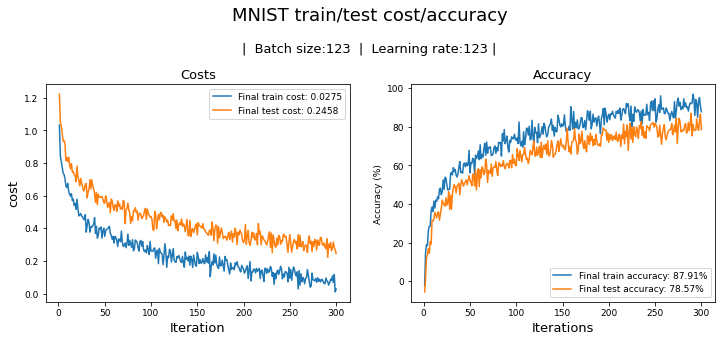
\includegraphics[width=0.8\textwidth]{cost_accuracy_per_iteration.png}
		\caption{Plot showing how the cost and accuracy, evaluated on the training and test sets, is changing with number of iterations. It can be seen that\ldots \textit{(note your curves will look different!)}}
		\label{fig:cost_per_iteration_linear}
	\end{figure}
	\hfill \break
	\textit{\textbf{Exercise 2b.} Plot weight matrices}
	
	\textit{Include the requested plot of the weight matrices and comment on the result. How can we interpret the results? Note, some weight matrices are clearer to interpret than others, why?}
	
	As we can see in Figure \ref{fig:weights}...
	
	
	\begin{figure}[H]
		\centering
		\begin{subfigure}[b]{0.24\textwidth}
			\centering
			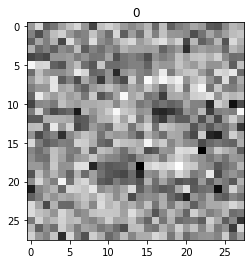
\includegraphics[width=\textwidth]{weights0}
		\end{subfigure}
		\begin{subfigure}[b]{0.24\textwidth}
			\centering
			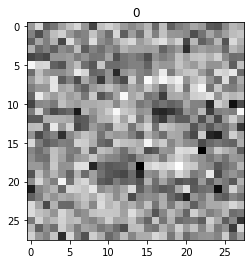
\includegraphics[width=\textwidth]{weights0}
		\end{subfigure}
		\begin{subfigure}[b]{0.24\textwidth}
			\centering
			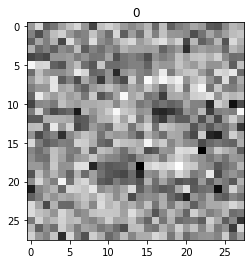
\includegraphics[width=\textwidth]{weights0}
		\end{subfigure}
		\begin{subfigure}[b]{0.24\textwidth}
			\centering
			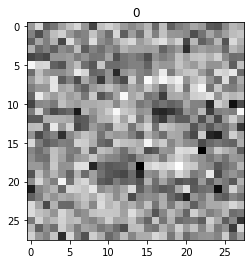
\includegraphics[width=\textwidth]{weights0}
		\end{subfigure}\\
		\caption{\textit{(your weight matrices will look different!)}}
		\label{fig:weights}
	\end{figure}
	
	
	\hfill \break
	\textit{\textbf{Exercise 3.} Evaluate your multi-layer neural network}
	
	\textit{Include the requested performance plot and comment on the result.
	Provide details on batch size, learning rate and model architecture (hidden units and activation function). Describe shortly how you came up with your design choices and if you tried other settings as well.}

	See Figure \ref{fig:cost_per_iteration_nn}.
	
	\begin{figure}[H]
		\centering
		\caption{Plot showing the cost and accuracy for multi-layer neural network....}
		\label{fig:cost_per_iteration_nn}
	\end{figure}	
	
	\hfill \break
	\textit{\textbf{Use of generative AI}}
	
	Write a few sentences if you have or have not used any generative AI, and if so how.
	
	
	
	\begin{thebibliography}{1}
		
		\bibitem{Adams} Adams, Douglas (1979). The Hitchhiker's Guide to the Galaxy. Pocket Books. p. 3.
		
	\end{thebibliography}
	
	\pagebreak
	
	\appendix
	\section{Code}
	\label{app:code}
	
	\inputminted[frame=lines,framesep=2mm,linenos]{python}{my_code.py}
	
\end{document}